% The research corpus (ci/research.json): Palatino (mathpazo) with
% Helvetica, a theorem-heavy mathematics paper with TikZ diagrams.
\documentclass[11pt]{article}
\usepackage[T1]{fontenc}
\usepackage[sc,osf]{mathpazo}
\usepackage[scaled=0.95]{helvet}
\usepackage{amsmath,amssymb,amsthm}
\usepackage{geometry}
\usepackage{tikz}
\usetikzlibrary{arrows.meta,positioning,matrix}
\usepackage[colorlinks=true,linkcolor=blue,citecolor=teal]{hyperref}
\newtheorem{theorem}{Theorem}[section]
\newtheorem{lemma}[theorem]{Lemma}
\theoremstyle{definition}
\newtheorem{definition}[theorem]{Definition}
\theoremstyle{remark}
\newtheorem*{remark}{Remark}
\title{\textsf{A Note on Commutative Diagrams}}
\author{E. Mathematician}
\date{2026}
\begin{document}
\maketitle
\section{Definitions}
\begin{definition}\label{def:functor}
A \emph{functor} $F\colon \mathcal{C} \to \mathcal{D}$ assigns to each
object $X$ an object $FX$ and to each arrow $f\colon X\to Y$ an arrow
$Ff\colon FX \to FY$, preserving identities and composition.
\end{definition}
\begin{lemma}\label{lem:square}
For a natural transformation $\eta\colon F \Rightarrow G$ the square
below commutes.
\end{lemma}
\begin{center}
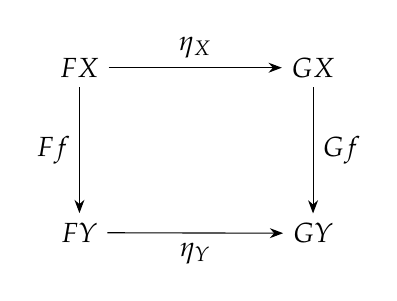
\begin{tikzpicture}[node distance=2.2cm, >={Stealth}]
  \node (FX) {$FX$};
  \node (GX) [right=of FX] {$GX$};
  \node (FY) [below=1.6cm of FX] {$FY$};
  \node (GY) [below=1.6cm of GX] {$GY$};
  \draw[->] (FX) -- node[above] {$\eta_X$} (GX);
  \draw[->] (FY) -- node[below] {$\eta_Y$} (GY);
  \draw[->] (FX) -- node[left] {$Ff$} (FY);
  \draw[->] (GX) -- node[right] {$Gf$} (GY);
\end{tikzpicture}
\end{center}
\begin{proof}
By definition, $\eta_Y \circ Ff = Gf \circ \eta_X$ for every
$f\colon X \to Y$.
\end{proof}
\section{A theorem}
\begin{theorem}[Yoneda]\label{thm:yoneda}
For a locally small $\mathcal{C}$, $\mathrm{Nat}(\mathrm{Hom}(A,-), F)
\cong F A$ naturally in $A$ and $F$.
\end{theorem}
\begin{remark}
Old-style figures 0123456789 and \textsc{Small Capitals} come from
mathpazo's options; $\int_0^\infty e^{-x^2}\,dx = \tfrac{\sqrt{\pi}}{2}$
and $\sum_{n\ge1} n^{-2} = \pi^2/6$ in Palatino's mathematics.
\end{remark}
Theorem~\ref{thm:yoneda} and Lemma~\ref{lem:square} are classical
\cite{lamport1994}.
\begin{align}
  \zeta(s) &= \sum_{n=1}^{\infty} \frac{1}{n^s} = \prod_{p} \frac{1}{1-p^{-s}}, \\
  \Gamma(z) &= \int_0^\infty t^{z-1} e^{-t}\, dt .
\end{align}
\bibliographystyle{alpha}
\bibliography{refs}
\end{document}
